\documentclass{article} % Класс печатного документа

% для поддержки русского языка
\usepackage[T2A]{fontenc} % поддержка специальных русских символов
\usepackage[utf8]{inputenc} % Кодировка исходного текста - utf8
\usepackage[english,russian]{babel} % Поддержка языка - русского с английским
\usepackage{indentfirst} % Отступ в первом абзаце

\usepackage{hyperref} % Для вставки гиперссылок
% \usepackage{listings} % Для вставки кусков кода
\usepackage{graphicx} % Вставка изображений
\usepackage{subfig} % Изображения друг напротив друга
\usepackage{float} % Для точного позиционирования картинок

% Default fixed font does not support bold face
\DeclareFixedFont{\ttb}{T1}{txtt}{bx}{n}{12} % for bold
\DeclareFixedFont{\ttm}{T1}{txtt}{m}{n}{12}  % for normal

% Custom colors
\usepackage{color}
\definecolor{deepblue}{rgb}{0,0,0.5}
\definecolor{deepred}{rgb}{0.6,0,0}
\definecolor{deepgreen}{rgb}{0,0.5,0}

\usepackage{listings}

% Python style for highlighting
\newcommand\pythonstyle{\lstset{
    language=Python,
    basicstyle=\ttm,
    otherkeywords={self},             % Add keywords here
    keywordstyle=\color{deepblue},
    emph={MyClass,__init__},          % Custom highlighting
    emphstyle=\color{deepred},    % Custom highlighting style
    stringstyle=\color{deepgreen},
    frame=tb,                         % Any extra options here
    showstringspaces=false,           % 
    basicstyle=\small,                % уменьшить размер шрифта
    columns=flexible                  % чтобы при копировании не было пробелов везде
}}


% Python environment
\lstnewenvironment{python}[1][]
{
\pythonstyle
\lstset{#1}
}
{}

% Python for external files
\newcommand\pythonexternal[2][]{{
\pythonstyle
\lstinputlisting[#1]{#2}}}

% Python for inline
\newcommand\pythoninline[1]{{\pythonstyle\lstinline!#1!}}

\makeatletter
\def\lst@outputspace{{\ifx\lst@bkgcolor\empty\color{white}\else\lst@bkgcolor\fi\lst@visiblespace}}
\makeatother
 % для красивого оформления python кода

% путь к папке с изображениями
\graphicspath{{./figs/}}

\title{Отчёт 9\protect\\
    Классификация.\\
    Метод метод случайного леса деревьев решений\\
    (random forest)} % заголовок документа
\author{Свичкарев А.\,В.} % Автор документа
\date{\today} % Текущая дата

\begin{document} % Конец преамбулы, начало текста

\maketitle % Печатает заголовок, список авторов и дату

\section{Цель}
Изучить способы решения задач классификации данных с
применением метода случайного леса деревьев решений (Random Forest).

\section{Задание №1}
Написать программу построения модели классификации
данных из файла
\verb$winequality-red.csv$ методом случайного леса деревьев решений
(Random Forest) и визуализации деревьев решений.
Построить и визуализировать частные модели деревьев,
на основе которых построить модель предсказания значений данных.
Привести значение минимального среднего квадрата ошибки
Minimum MSE и график зависимости среднего квадрата ошибок (mean squared error - MSE) от числа деревьев в ансамбле.
Оценить точность предсказания при различных значениях параметров
numTreesMax, treeDepth, nAtt.
\bigskip

Реализация на основе кода программы из Приложения (файл \verb$exercise1.py$):
\pythonexternal{../exercise1.py}
\bigskip

Примеры частных моделей деревьев:
\begin{figure}[H]
	\centering
	\subfloat[Первое дерево]{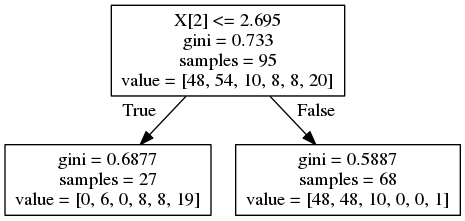
\includegraphics[width=0.5\textwidth]{tree1Ex1.png}}
	\hfill
	\subfloat[Второе дерево]{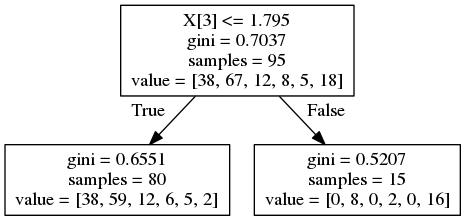
\includegraphics[width=0.5\textwidth]{tree2Ex1.png}}
    \caption{Графические построения деревьев}
\end{figure}
\bigskip

\clearpage
Значение минимального среднего квадрата ошибки Minimum MSE
при различных параметрах (закодированы в названиях файлов):
\lstinputlisting{./ex1_output.txt}

\begin{figure}[H]
	\centering
	\subfloat[mseEx1\_ntm30td1na4]{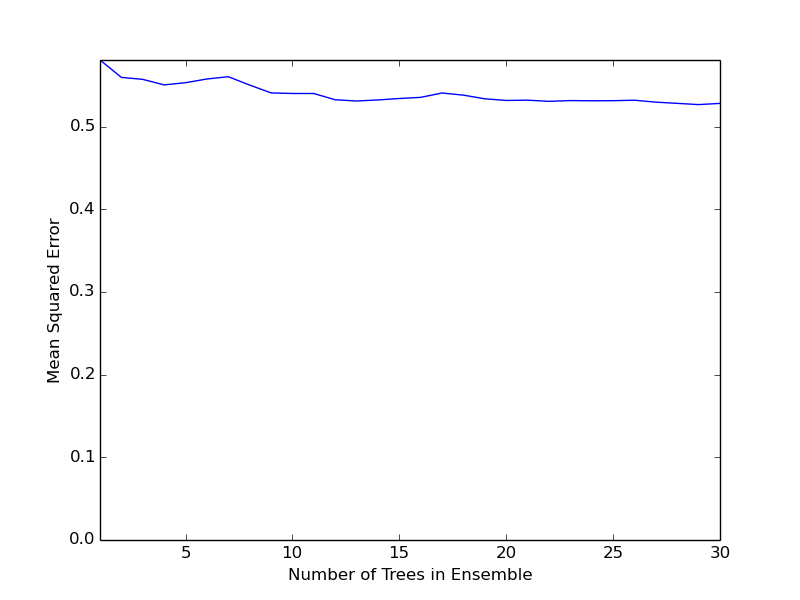
\includegraphics[width=0.5\textwidth]{mseEx1_ntm30td1na4}}
	\hfill
	\subfloat[mseEx1\_ntm30td1na3]{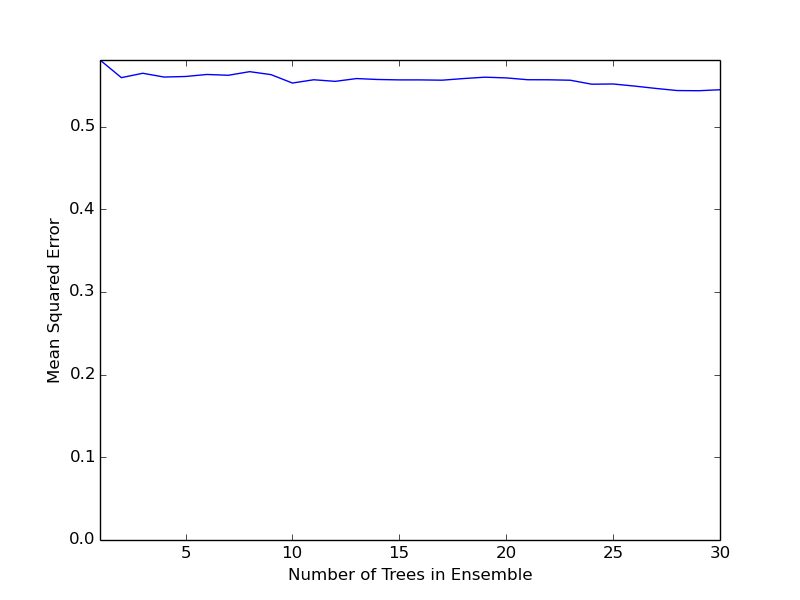
\includegraphics[width=0.5\textwidth]{mseEx1_ntm30td1na3}}
\end{figure}
\begin{figure}[H]
	\centering
	\subfloat[mseEx1\_ntm30td1na1]{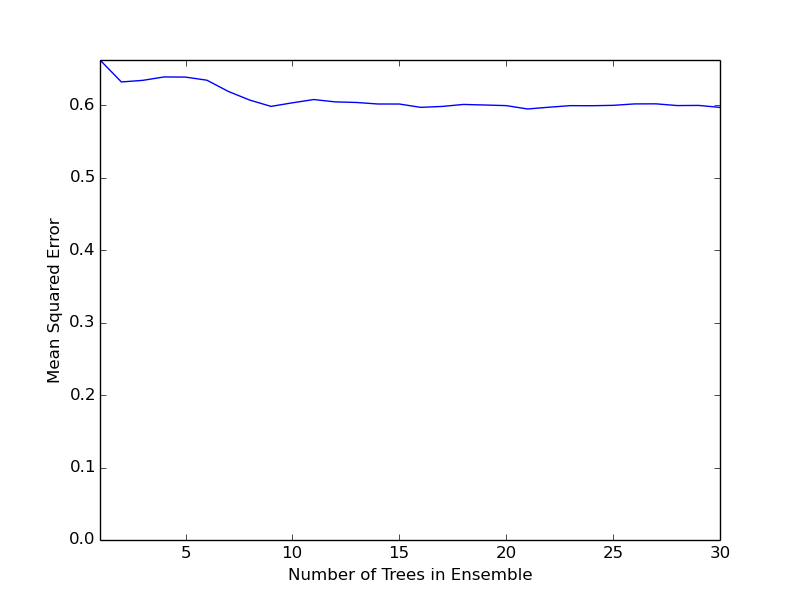
\includegraphics[width=0.5\textwidth]{mseEx1_ntm30td1na1}}
	\hfill
	\subfloat[mseEx1\_ntm60td1na4]{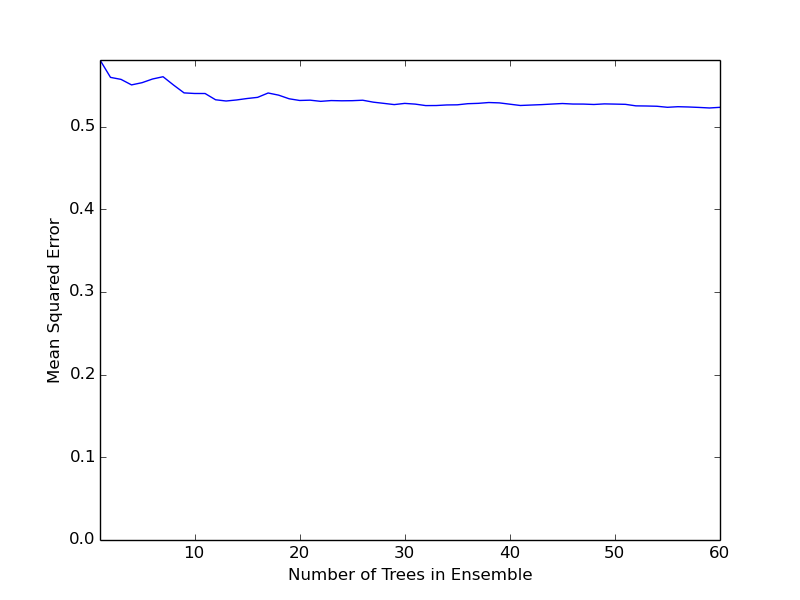
\includegraphics[width=0.5\textwidth]{mseEx1_ntm60td1na4}}
\end{figure}
\begin{figure}[H]
	\centering
	\subfloat[mseEx1\_ntm90td1na4]{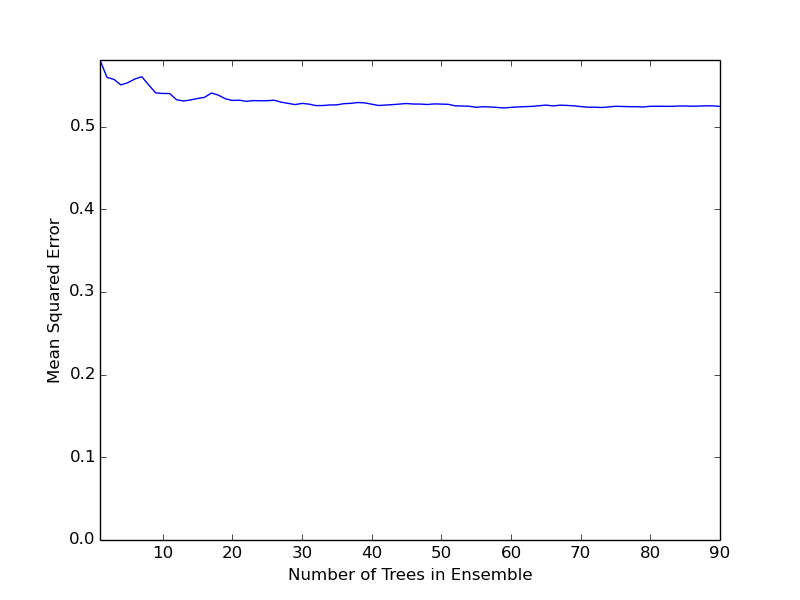
\includegraphics[width=0.5\textwidth]{mseEx1_ntm90td1na4}}
	\hfill
	\subfloat[mseEx1\_ntm30td3na4]{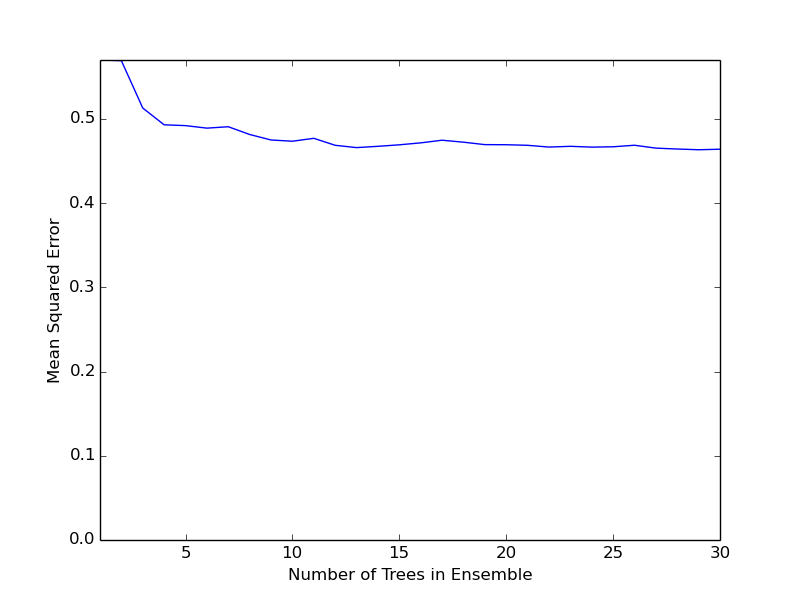
\includegraphics[width=0.5\textwidth]{mseEx1_ntm30td3na4}}
\end{figure}
\begin{figure}[H]
	\centering
	\subfloat[mseEx1\_ntm30td13na4]{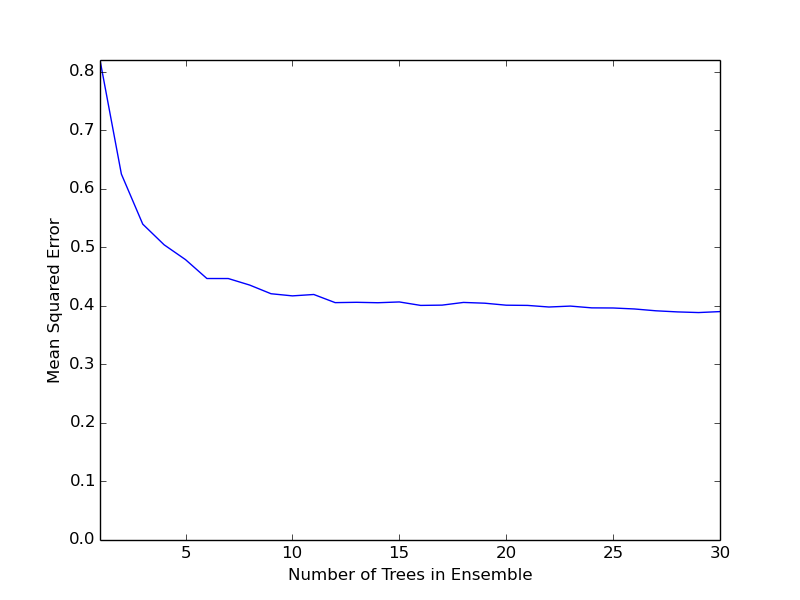
\includegraphics[width=0.5\textwidth]{mseEx1_ntm30td13na4}}
	\hfill
	\subfloat[mseEx1\_ntm30td20na4]{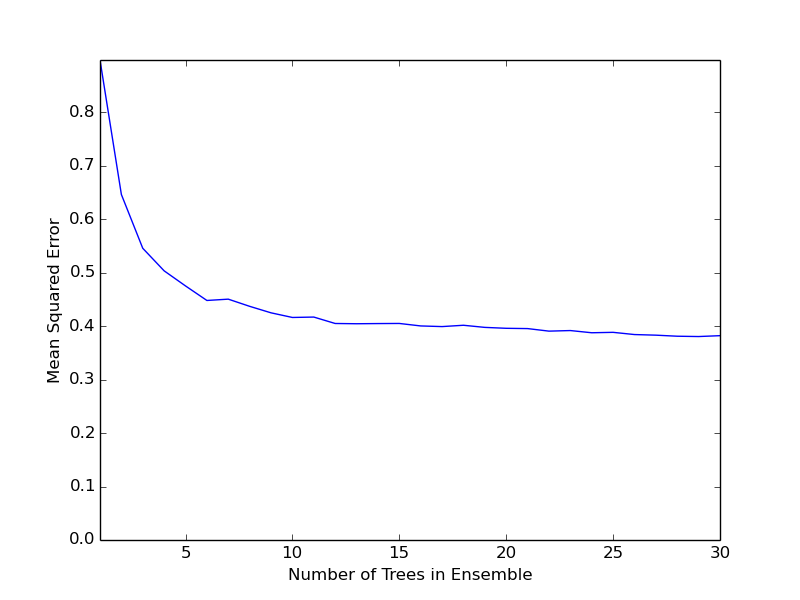
\includegraphics[width=0.5\textwidth]{mseEx1_ntm30td20na4}}
\end{figure}
\bigskip

Среди протестированных комбинаций минимум ошибки достигается
при размере ансамбля в 30 деревьев,
глубине дерева 20 и выборки в 4 признака для каждого дерева.

\clearpage
\section{Задание №2}
Выполнить классификацию данных из файла
\verb$breast-cancer-wisconsin.data.csv$ методом
методом случайного леса деревьев решений (Random Forest) и визуализировать деревья
решений. Привести результаты предсказания значений данных. Оценить точность
предсказания при различных значениях параметров numTreesMax, treeDepth, nAtt.
\bigskip

Реализация на основе кода программы из Приложения (файл \verb$exercise2.py$):
\pythonexternal{../exercise2.py}
\bigskip

\clearpage
Примеры частных моделей деревьев:
\begin{figure}[H]
	\centering
	\subfloat[Первое дерево]{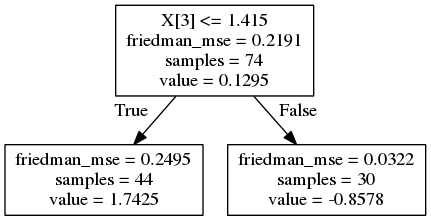
\includegraphics[width=0.5\textwidth]{tree1Ex2.png}}
	\hfill
	\subfloat[Второе дерево]{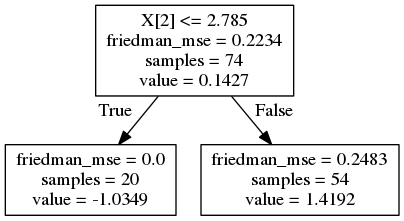
\includegraphics[width=0.5\textwidth]{tree2Ex2.png}}
    \caption{Графические построения деревьев}
\end{figure}
\bigskip

Значение минимального среднего квадрата ошибки Minimum MSE
при различных параметрах (закодированы в названиях файлов):
\lstinputlisting{./ex2_output.txt}

\begin{figure}[H]
	\centering
	\subfloat[mseEx2\_ntm30td2na3]{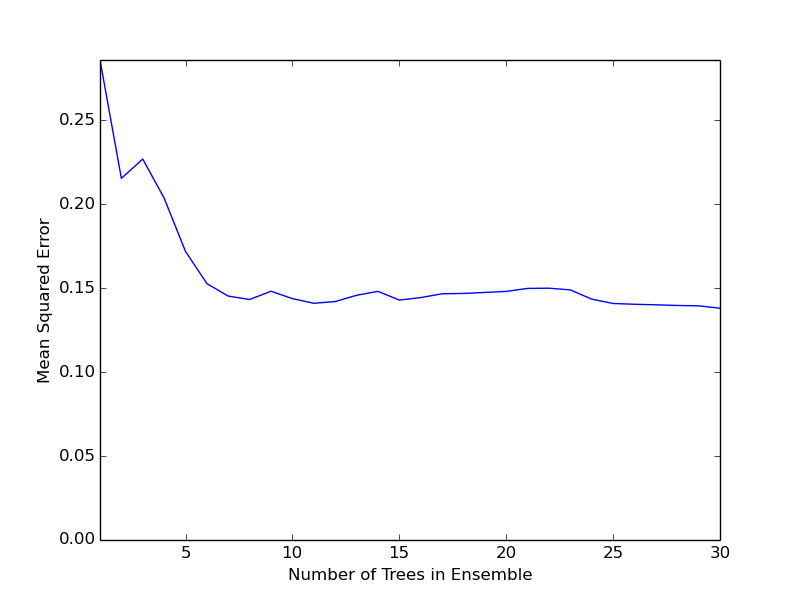
\includegraphics[width=0.5\textwidth]{mseEx2_ntm30td2na3}}
	\hfill
	\subfloat[mseEx2\_ntm30td5na3]{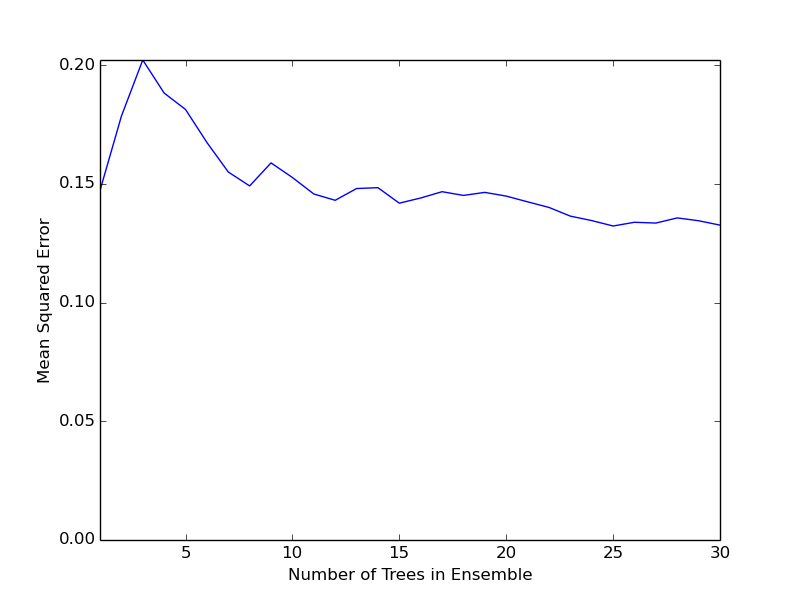
\includegraphics[width=0.5\textwidth]{mseEx2_ntm30td5na3}}
\end{figure}
\begin{figure}[H]
	\centering
	\subfloat[mseEx2\_ntm90td5na3]{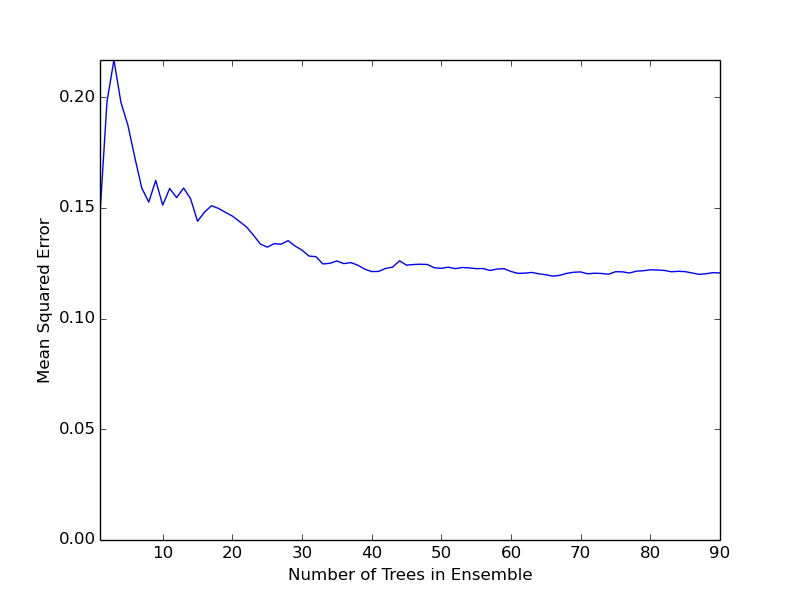
\includegraphics[width=0.5\textwidth]{mseEx2_ntm90td5na3}}
	\hfill
	\subfloat[mseEx2\_ntm90td5na4]{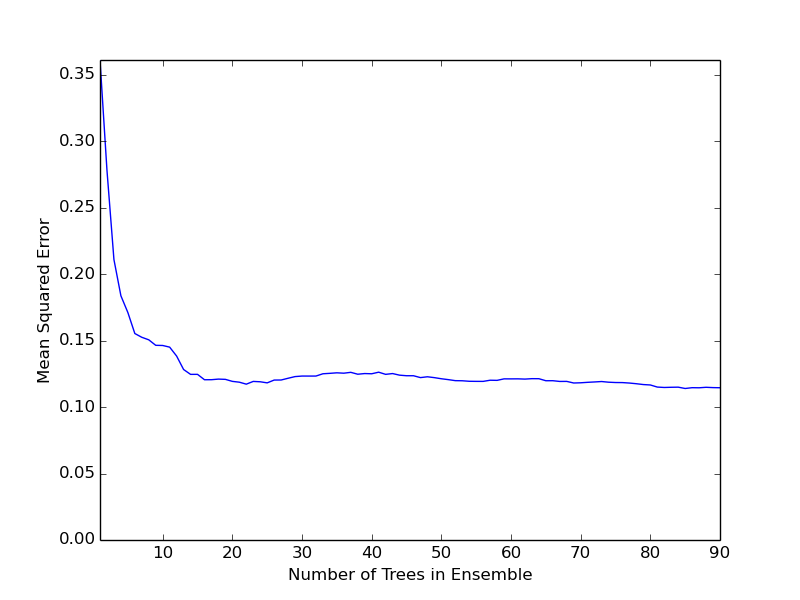
\includegraphics[width=0.5\textwidth]{mseEx2_ntm90td5na4}}
\end{figure}
\begin{figure}[H]
	\centering
	\subfloat[mseEx2\_ntm90td5na5]{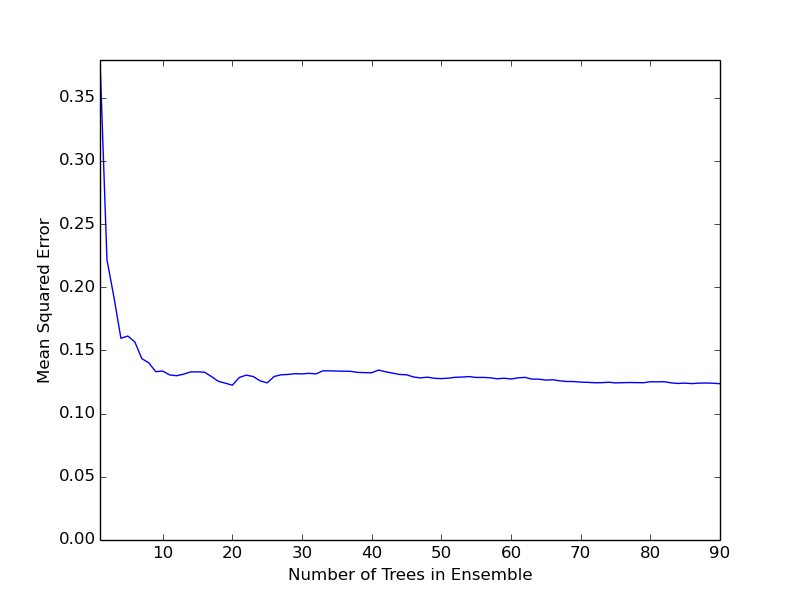
\includegraphics[width=0.5\textwidth]{mseEx2_ntm90td5na5}}
	\hfill
	\subfloat[mseEx2\_ntm90td12na4]{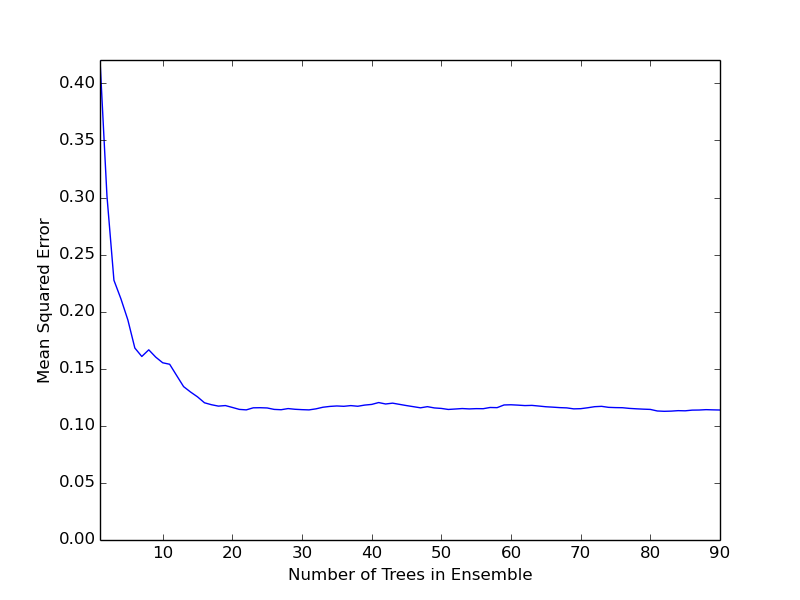
\includegraphics[width=0.5\textwidth]{mseEx2_ntm90td12na4}}
\end{figure}
\begin{figure}[H]
	\centering
	\subfloat[mseEx2\_ntm90td20na4]{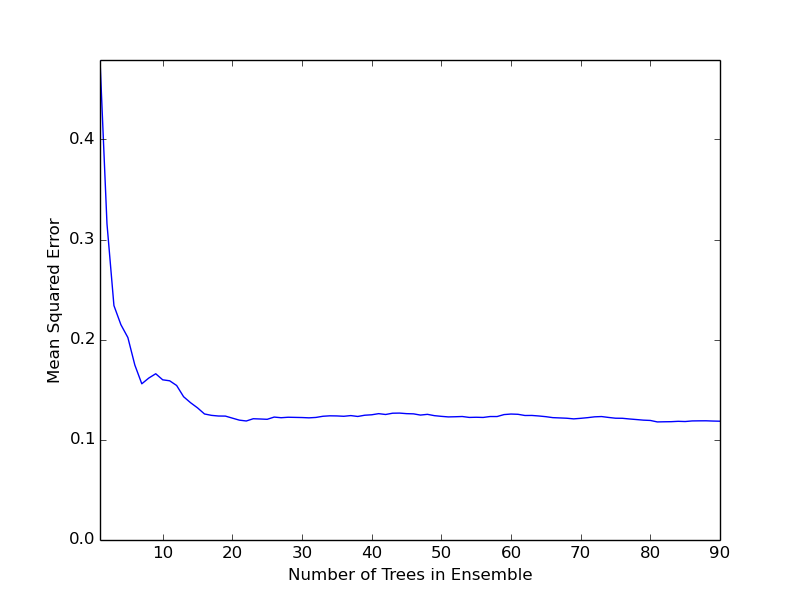
\includegraphics[width=0.5\textwidth]{mseEx2_ntm90td20na4}}
	\hfill
	\subfloat[mseEx2\_ntm90td2na3]{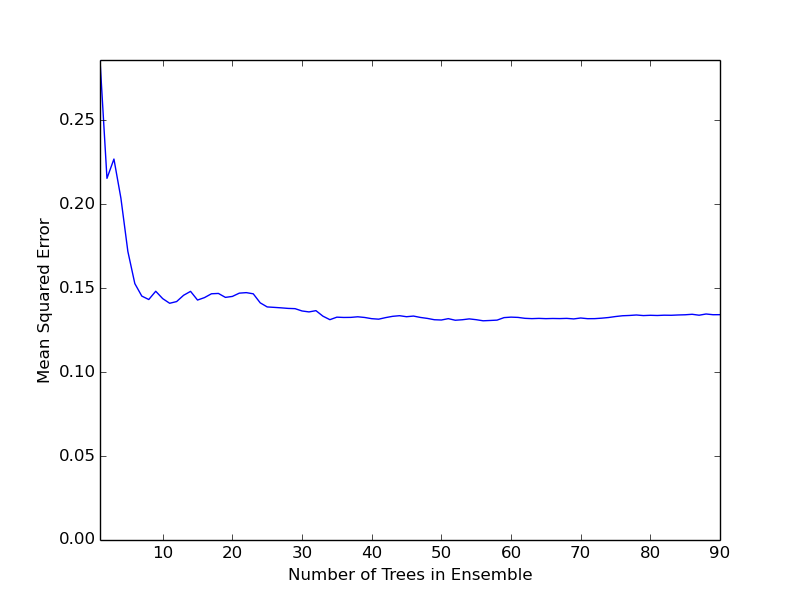
\includegraphics[width=0.5\textwidth]{mseEx2_ntm90td2na3}}
\end{figure}
\bigskip

Среди протестированных комбинаций минимум ошибки достигается
при размере ансамбля в 90 деревьев,
глубине дерева 12 и выборки в 4 признака для каждого дерева.

На самом деле данная реализация
не является в чистом виде random forest,
потому что в оригинальном алгоритме
в построение для каждого узла выбираются
своя выборка атрибутов.
Этот алгоритм правильнее было бы назвать
баггинг с случайным выбором признаков.
Данное несоответствие вызвано
невозможностью реализовать данную функциональность
через DecisionTreeRegressor.

\section{Пояснение}
Исходный код доступен по ссылке:
\href{https://github.com/SvichkarevAnatoly/Course-Python-Bioinformatics/tree/master/semester2/task9}
{github.com}

\end{document} % Конец документа
